\chapter{}

\begin{figure}
\centering
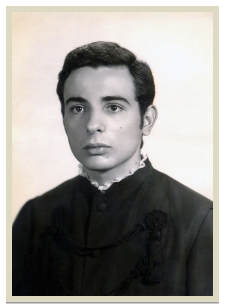
\includegraphics[width=0.8\linewidth]{17/paulo-formatura.png}
\caption{Paulo no dia da formatura.}
\end{figure}

Paulo formou-se em meados do ano de 1971 e foi trabalhar no Mato Grosso, na cidade de Campo Grande, num escritório de planejamento agrícola.
Marcamos nosso casamento para outubro daquele mesmo ano.
Transferi-me de volta para Araraquara, para ajudar minha mãe nas providências necessárias, uma vez que ela já estava envolvida com o casamento da minha irmã, marcado para apenas três meses antes do meu.


Não importa o que se diga a respeito do casamento, da sua sobrevivência enquanto instituição, a verdade inegável é que a cerimônia ainda é um momento de sonho na vida da maioria das mulheres.
Decidi que ia vivê-lo em toda sua plenitude e quis parecer bonita nesse dia como nunca antes.
Escolhi cuidadosamente cada item da festa, do vestido ao cardápio, passando pela música e pela decoração da pequena capela.
Paulo e eu queríamos uma cerimônia discreta, para poucas pessoas, para alívio dos meus pais.
O casamento da minha irmã assumiu proporções orientais, uma vez que ambas as famílias eram radicadas em Araraquara há muito tempo e por isso não houve como escapar de convidar meio mundo.

Ao anoitecer do dia dez de outubro de mil novecentos e setenta e um, ao entrar pelo braço do meu pai naquela capelinha e ouvir o murmúrio de admiração das pessoas ali reunidas, comecei a flutuar em direção ao altar.
Senti-me no centro de um palco iluminado.
Tudo o resto era figuração.
Inclusive o noivo, como confessei a ele mais tarde, depois da festa.


\begin{figure}[H]
\centering
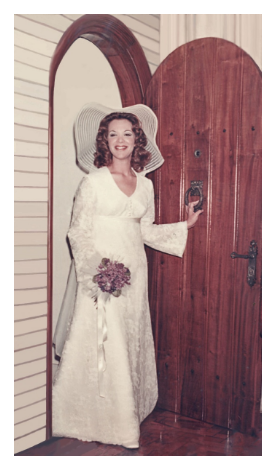
\includegraphics[width=0.5\linewidth]{17/vestida-casar.png}
\caption{Vestida para casar.}
\end{figure}

Em toda a minha história de vida naquela cidade, minhas aparições públicas tinham sido repetidamente um desastre.
Eu sempre fui o tipo de pessoa que escorrega no degrau, derruba a louça, esbarra nos móveis, pisa no pé do parceiro e esquece o discurso.
Na minha derradeira atuação, na formatura do curso colegial, tropecei no fio do microfone e, levando o dito cujo de cambulhada, ameacei varrer da mesa de honra todos os diplomas ali empilhados, na tentativa de me segurar, até que consegui finalmente me agarrar à mão de quem?  Dele mesmo, do meu algoz, o esquálido professor de Matemática que por pouco não rolou comigo num abraço solidário, palco abaixo.
A assistência foi ao delírio.
 

Mas, no dia do meu casamento, se, ao invés daquela minúscula nave, eu tivesse que palmilhar os tapetes de Westminster, eu o faria, com certeza, sem baixar o olhar uma única vez.
Ao longo da vida tenho recomendado às mocinhas que não dispensem a cerimônia de casamento.
Talvez não tenham outra oportunidade de se sentirem tão lindas como nesse dia.

\begin{figure}[H]
\centering
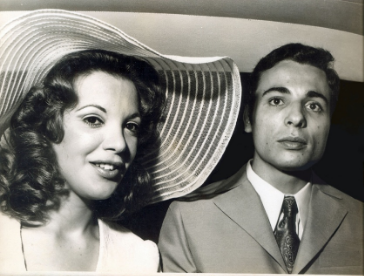
\includegraphics[width=0.75\linewidth]{17/no-carro.png}
\caption{No carro, já casados, a caminho da recepção.}
\end{figure}

Terminada a festa, partimos em lua de mel para o Rio Grande do Sul e, de lá, para Campo Grande, onde se desenrolaria a etapa inicial da nossa vida de casados.

Paulo tinha alugado um pequeno apartamento no centro, próximo ao escritório onde trabalhava.
Ganháramos um bocado de presentes e certa quantia em dinheiro da família dele, de modo que pude deixar tudo bem bonitinho, até com cortinas e todo o necessário para uma rotina doméstica confortável e aconchegante.
Descobri que tomar conta de casa me dava um insuspeitado prazer.
Gosto disso até hoje.
Só não contava com a inquietação do Paulo.
